\section{Configuration Panel}
\label{sec:osgview_config_panel}

\begin{figure}[H]
    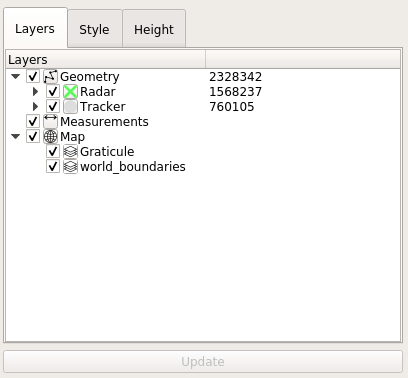
\includegraphics[width=8cm,frame]{../screenshots/osgview_config_panel.png}
  \caption{OSG View configuration panel}
\end{figure}

There exist 3 tabs:
\begin{itemize}
 \item Layers: Allows configuration what data is shown, and access to the map and measurement functions
 \item Style: Allows configuration how data is shown
 \item Height: Allows configuration of the height usage in the shown geometry
\end{itemize}
\ \\

Additionally, at the bottom the 'Update' button allows redraw/reloading of the geometry data. This button becomes available if changes in the Style or Height tabs require a redraw or a reload of the data. \\

\subfile{osg_layers_tab}
\subfile{osg_style_tab} 
\subfile{osg_height_tab} 
